\documentclass{standalone}
\begin{document}
	\subsection{Gold Standard}
	
	In this section I will discuss the quantitative match between the achieved segmentation and the gold standard. The gold stantrd used involves $5$ semiautomatic segmentation made by a certified software and refined and checked by experts. This segmentation was provided by the Department of Diagnostic and Preventive Medicine of the Poloclinico Sant'Orsola - Malpighi.\\
	The comparison was made for all the scans by Dice similarity coefficient.\\
	To define this kind of metric we consider the segmentation labels as a boolean mask, in which $True$ corresponds to the identified lesion area, and $False$ to other areas. This mask is compared to the actual ground truth, given by the gold standard, so we are able to compute the True positives (TP), True negative (TN), false positives(FP) and false negatives(FN) rate. Once we have computed these quantities, we are able to compute the dice score coefficient, given by :  
	\begin{equation}
		DSC = \frac{2TP}{2TP + FP + FN}
	\end{equation}

	This coefficient, which is in $[0, 1]$, will provide a measure of the goodness of the segmentation.\\ Dica coefficient were computed for all the five patients and the results are reported in table\,\ref{tab:DSC}. 
	
	\begin{table}[h!]
		\centering
		\begin{tabular}{|c|c|c|c|c|c|}
			\hline
				  &DSC		&TP	($\%$)	&TN	($\%$)&FP($\%$)	&FN	($\%$)	\\ \hline
		Patient 1 &	$0.519$	& $0.033$	& $99.90$ &	$0.048$	& $0.014$	\\
		Patient 2 & $0.559$	& $0.417$	& $98.93$ &	$0.031$	& $0.627$	\\
		Patient 3 &	$0.708$	& $0.649$	& $98.82$ & $0.045$	& $0.489$	\\
		Patient 4 &	$0.546$	& $0.0298$	& $99.92$ &	$0.021$	& $0.028$	\\
		Patient 5 &	$0.765$	& $0.269$	& $99.56$ &	$0.006$	& $0.159$	\\ \hline

		\end{tabular}\caption{Table of the dice coefficient for each gold standard patient. The accurate manual segmentation was takes as ground truth. }\label{tab:DSC}
	\end{table}

	The first thing that we can notice is that the percentage of the true negative is much higher than the other.; that because the number of pixels concerning the labeled object would be very few against the number of pixels related to the background.\\ An other thing we can notice is that not all the patient have similar agreement: Patient 1, 2, and 4 show DSC near the $0.55$, the remaining two near $0.73$. This may be caused to the fact that the chosen patients presents different severity of the disease and lesion characteristics: as we will see the developed method performs well in case of normal or severe lesions, but have some difficult in case of low contrast between lesions and normal lung regions.
	 	
 		\begin{figure}[h!]
 		\centering
 				\subfigure[Ground truth for Axial, sagittal and coronal view of the first patient]
 				{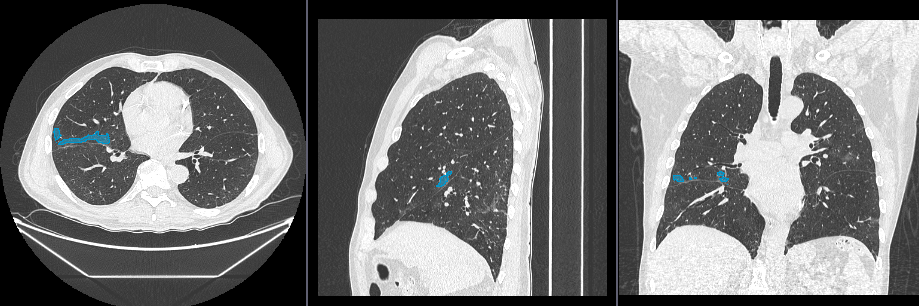
\includegraphics[scale=.4]{PATIENT1_GT.png}}
 		%\hspace{1mm}
 				\subfigure[Predicted lesions areas for Axial, sagittal and coronal view of the first patient]
 				{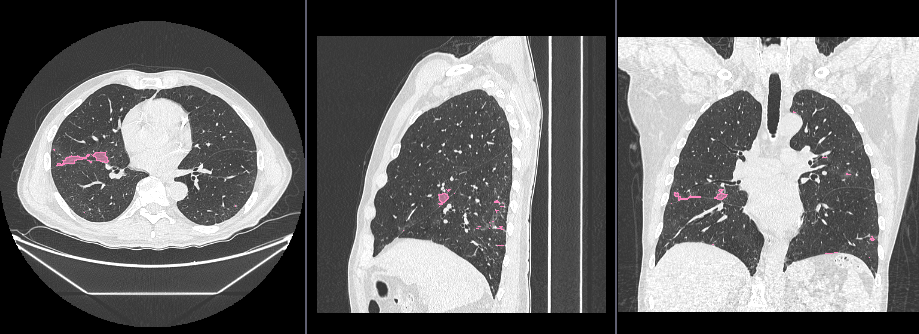
\includegraphics[scale=.4]{PATIENT1_PR.png}}
 			\caption{Comparison between the gold standard segmentation(blue) and the pipeline results(pink) for axial, sagittal and coronal view of a patient with a low involvement of lung parenchima. We can see that te main lesion areas are identified, even if an understimation of the total volume is present together with some small misclassified points.}\label{fig:pat1}
 		\end{figure}
 	
 	In \figurename\,\ref{fig:pat1} I've reported a comparison between the ground truth (blue) and the pipeline segmentation (pink) for the first patient in axial, sagittal and coronal view. We can see how the main lesion areas are correctly identified, however a low underestimation of the total lesion volume is presents, toghether with the presence of false positives in the lowest back regions.\\ This is a particular case, since the involvement of lung parenchima is very low, as is the contrast between lesions and healthy lung.\\
 	
 	
 		\begin{figure}[h!]
 			\centering
 				\subfigure[Ground truth for Axial, sagittal and coronal view of the third patient]
 						{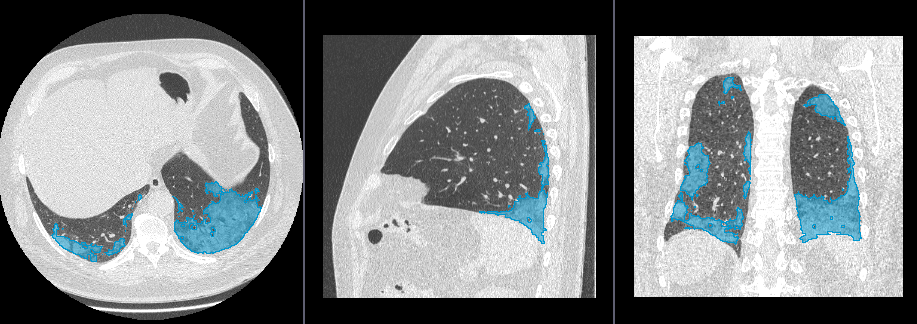
\includegraphics[scale=.4]{PATIENT3_GT.png}}
 		%\hspace{1mm}
 				\subfigure[Predicted lesions areas for Axial, sagittal and coronal view of the third patient]
 						{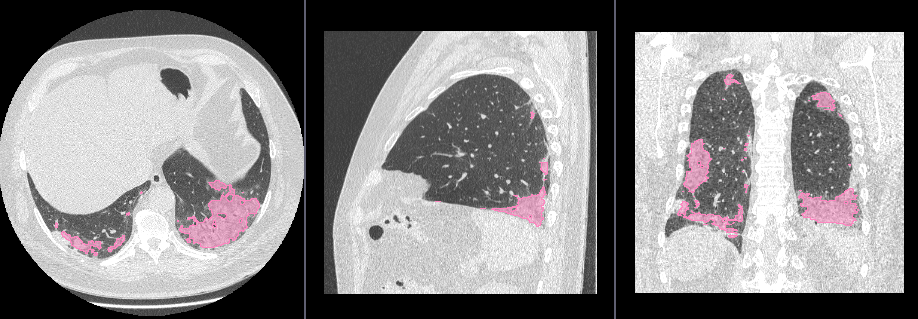
\includegraphics[scale=.4]{PATIENT3_PR.png}}
 		\caption{Comparison between the gold standard segmentation(blue) and the pipeline results(pink) for axial, sagittal and coronal view for a patient with a large involvement of lung parenchima. We can see how the lesion areas are correctly identified}\label{fig:pat3}
 		\end{figure}
 	
 	In \figurename\,\ref{fig:pat3} I've reported a comparison between the ground truth (blue) and the pipeline segmentation (pink) for the third patient in axial, sagittal and coronal view. The patient presents an high involvement of lung regions.  The lesion areas, which  in this case presents an high contrast with the lung regions, are correctly selected. In this case no misclassified points are detected, which is in agreement with the percentage detected by the dice score.
 	
 	
	
\end{document}